% Editable native annotations around unchanged verified IDE photographs.
\par
\begin{figure}[htbp]
  \centering
  \sbox0{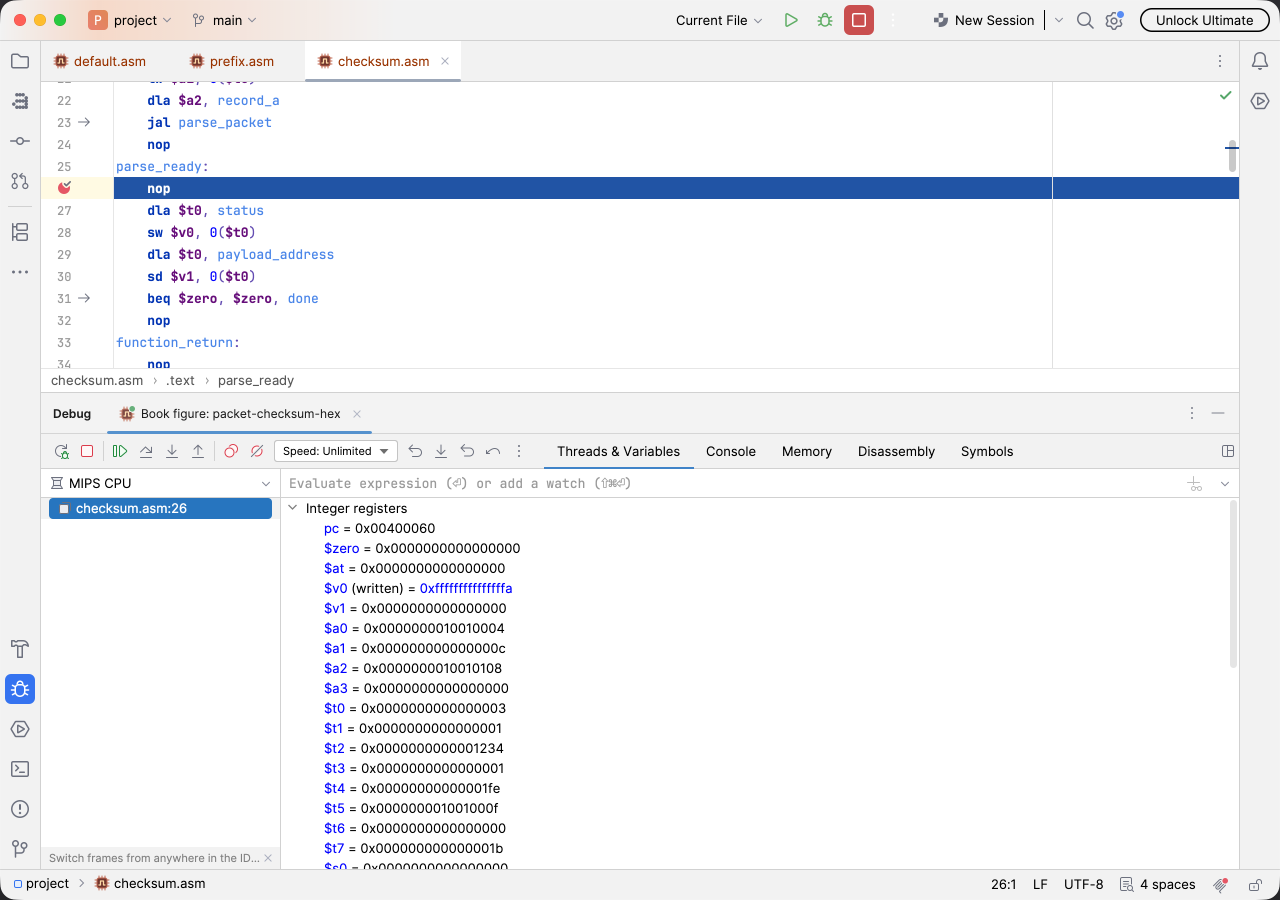
\includegraphics[artifact]{packages/013-binary-packet-parser/captures/f03-checksum/hex.png}}
  \sbox2{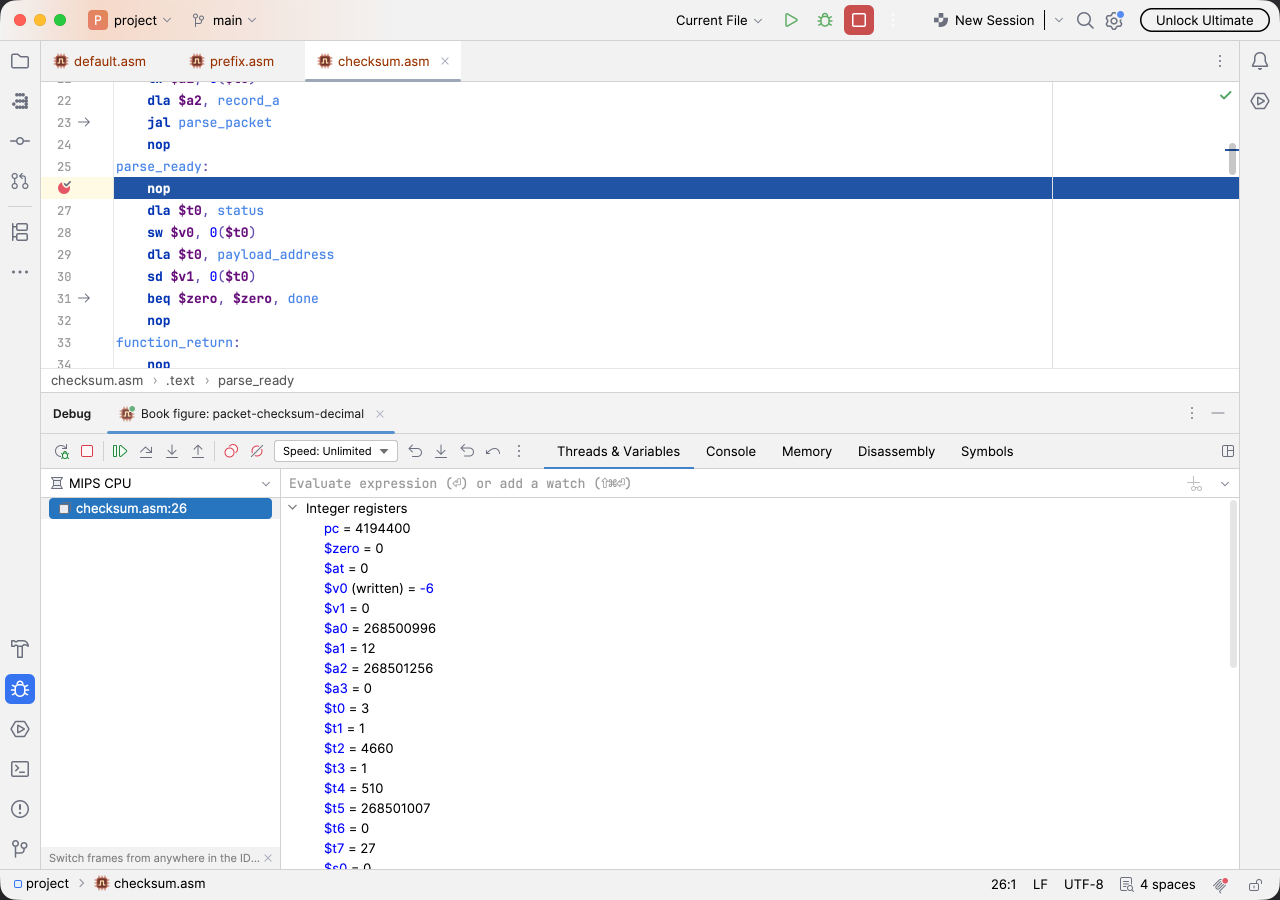
\includegraphics[artifact]{packages/013-binary-packet-parser/captures/f03-checksum/decimal.png}}
  \sbox4{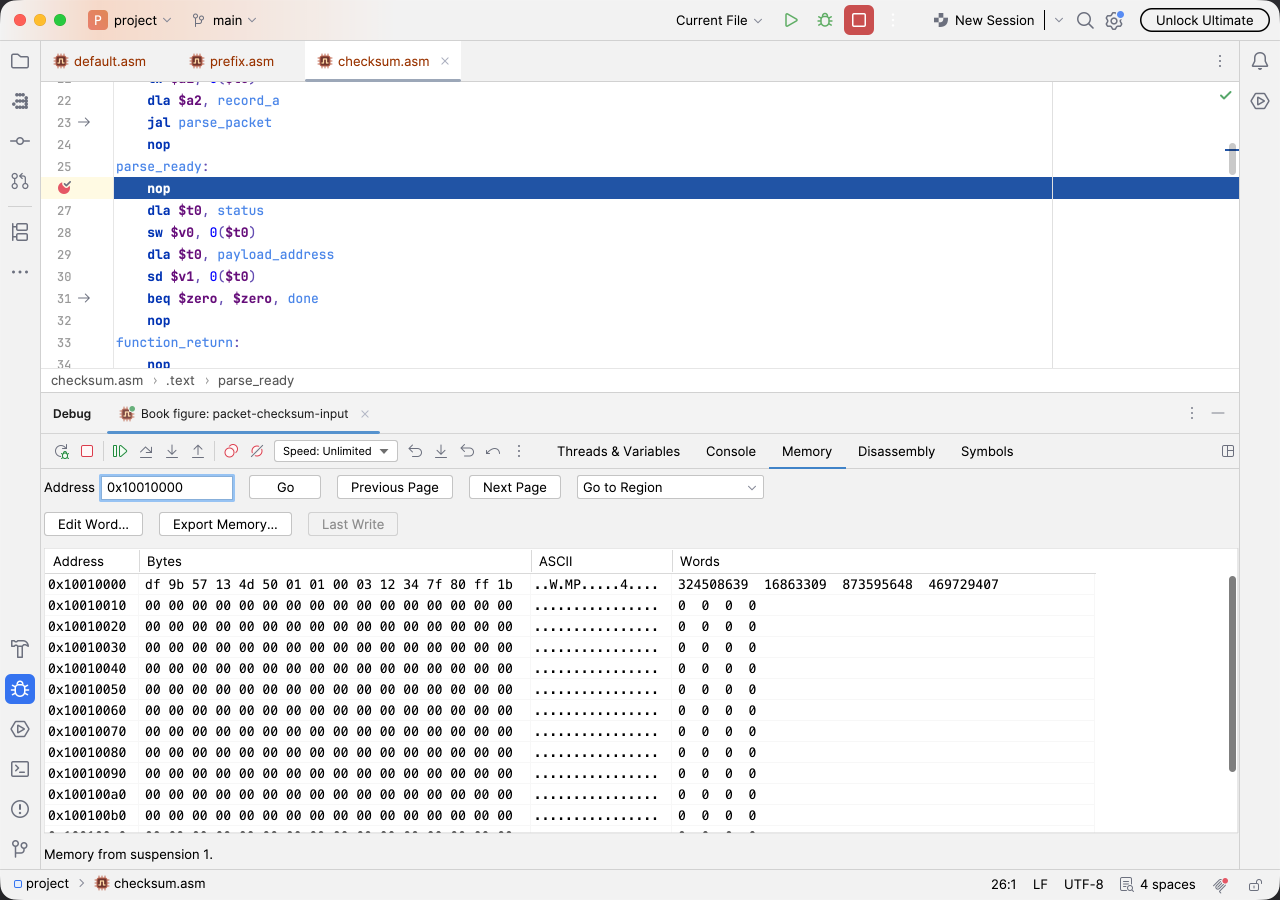
\includegraphics[artifact]{packages/013-binary-packet-parser/captures/f03-checksum/input.png}}
  \sbox6{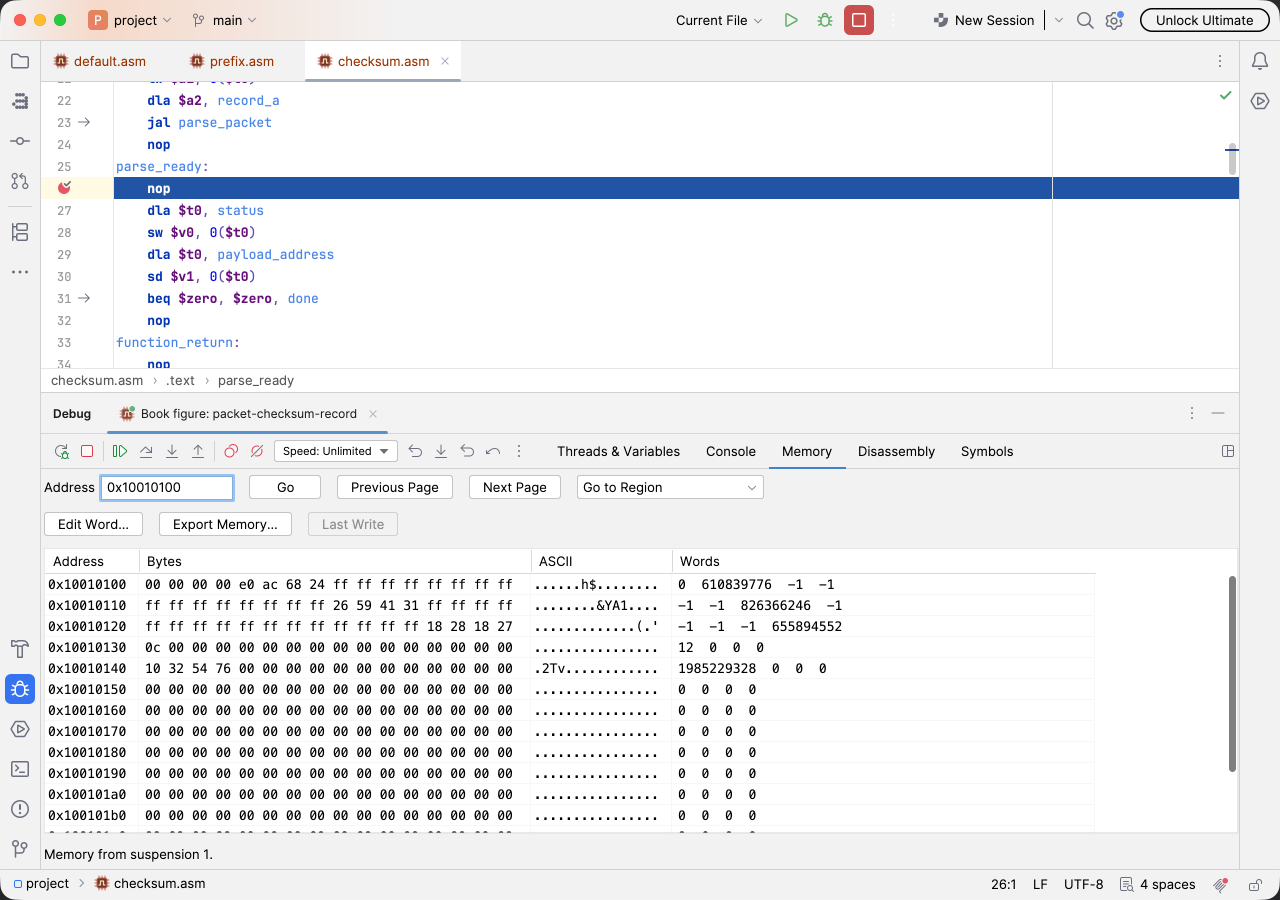
\includegraphics[artifact]{packages/013-binary-packet-parser/captures/f03-checksum/record.png}}
  \edef\MARSpacketchecksumsourceLeft{\the\dimexpr0.036718750\wd0\relax}
  \edef\MARSpacketchecksumsourceBottom{\the\dimexpr0.774444444\ht0\relax}
  \edef\MARSpacketchecksumsourceRight{\the\dimexpr0.713281250\wd0\relax}
  \edef\MARSpacketchecksumsourceTop{\the\dimexpr0.147777778\ht0\relax}
  \edef\MARSpacketchecksumhexLeft{\the\dimexpr0.246093750\wd0\relax}
  \edef\MARSpacketchecksumhexBottom{\the\dimexpr0.245555556\ht0\relax}
  \edef\MARSpacketchecksumhexRight{\the\dimexpr0.553906250\wd0\relax}
  \edef\MARSpacketchecksumhexTop{\the\dimexpr0.640000000\ht0\relax}
  \edef\MARSpacketchecksumdecimalLeft{\the\dimexpr0.246093750\wd2\relax}
  \edef\MARSpacketchecksumdecimalBottom{\the\dimexpr0.312222222\ht2\relax}
  \edef\MARSpacketchecksumdecimalRight{\the\dimexpr0.553906250\wd2\relax}
  \edef\MARSpacketchecksumdecimalTop{\the\dimexpr0.640000000\ht2\relax}
  \edef\MARSpacketchecksuminputLeft{\the\dimexpr0.034375000\wd4\relax}
  \edef\MARSpacketchecksuminputBottom{\the\dimexpr0.334444444\ht4\relax}
  \edef\MARSpacketchecksuminputRight{\the\dimexpr0.584375000\wd4\relax}
  \edef\MARSpacketchecksuminputTop{\the\dimexpr0.608888889\ht4\relax}
  \edef\MARSpacketchecksumrecordLeft{\the\dimexpr0.034375000\wd6\relax}
  \edef\MARSpacketchecksumrecordBottom{\the\dimexpr0.311111111\ht6\relax}
  \edef\MARSpacketchecksumrecordRight{\the\dimexpr0.584375000\wd6\relax}
  \edef\MARSpacketchecksumrecordTop{\the\dimexpr0.608888889\ht6\relax}
  \begin{tikzpicture}[alt={Five annotated details after validating a complete packet with a corrupted checksum. Available count is twelve. Only the final trailer changes from 0x1a to 0x1b. Native signed status is minus six and the payload pointer is zero. The four record A words retain their initial minus-one values; execution tracing establishes no stores to the record.}]
    \node[anchor=north west,inner sep=0,font=\small\bfseries] (source-title) at (6mm,0) {Next instruction after return};
    \node[anchor=north west,inner sep=0] (source) at ([yshift=-1mm]source-title.south west) {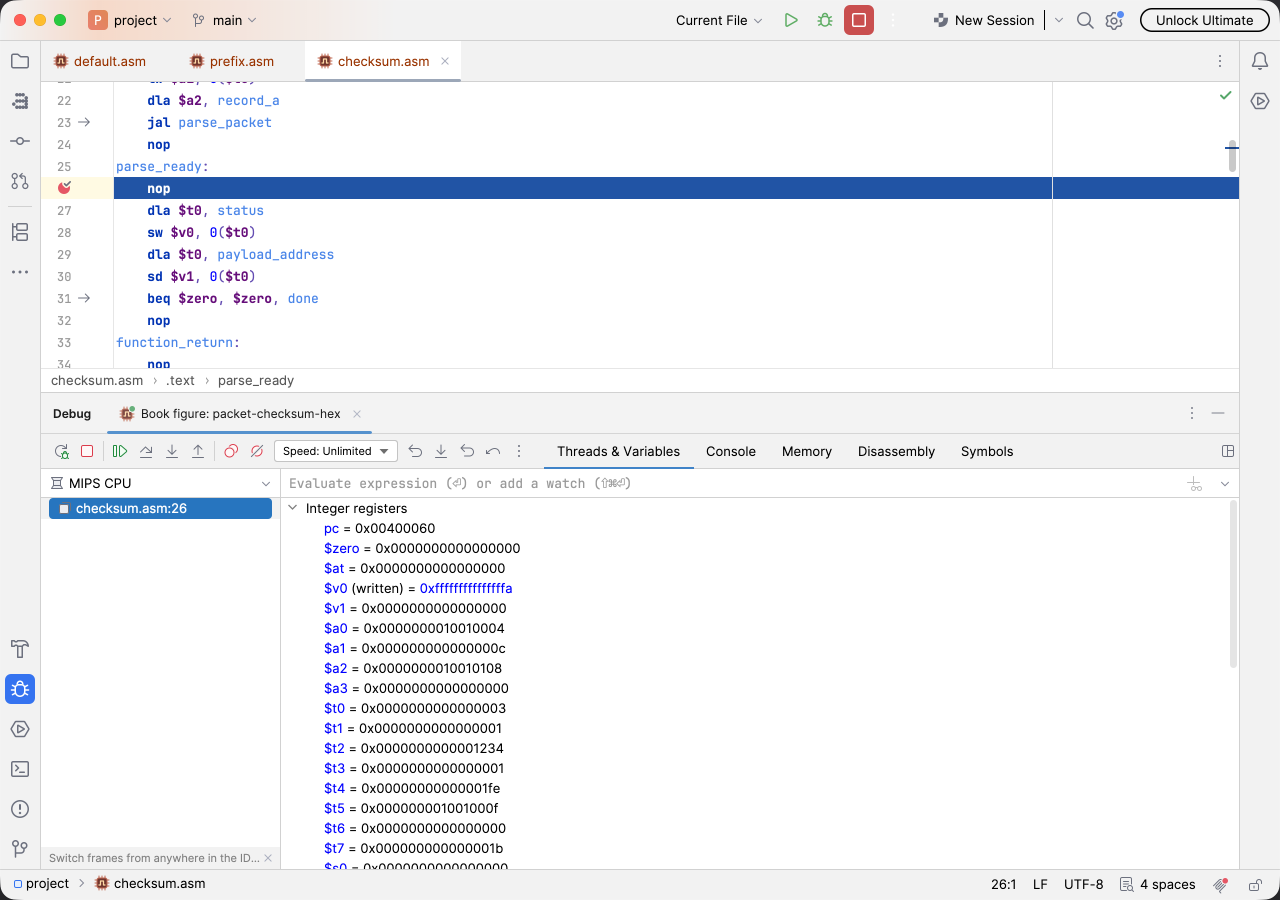
\includegraphics[width=0.54\linewidth,artifact,trim={\MARSpacketchecksumsourceLeft{} \MARSpacketchecksumsourceBottom{} \MARSpacketchecksumsourceRight{} \MARSpacketchecksumsourceTop{}},clip]{packages/013-binary-packet-parser/captures/f03-checksum/hex.png}};
    \begin{scope}[shift={(source.south west)},x={($(source.south east)-(source.south west)$)},y={($(source.north west)-(source.south west)$)}]
      \draw[black,line width=0.7pt] (0.215625000,0.057142857) rectangle (0.384375000,0.371428571);
      \node[draw=black,fill=white,circle,inner sep=1.5pt,font=\footnotesize] at ($(0.215625000,0.371428571)+(-3mm,0)$) {1};
    \end{scope}
    \node[anchor=north west,inner sep=0,font=\small\bfseries] (hex-title) at ([yshift=-3mm]source.south west) {Hexadecimal registers};
    \node[anchor=north west,inner sep=0] (hex) at ([yshift=-1mm]hex-title.south west) {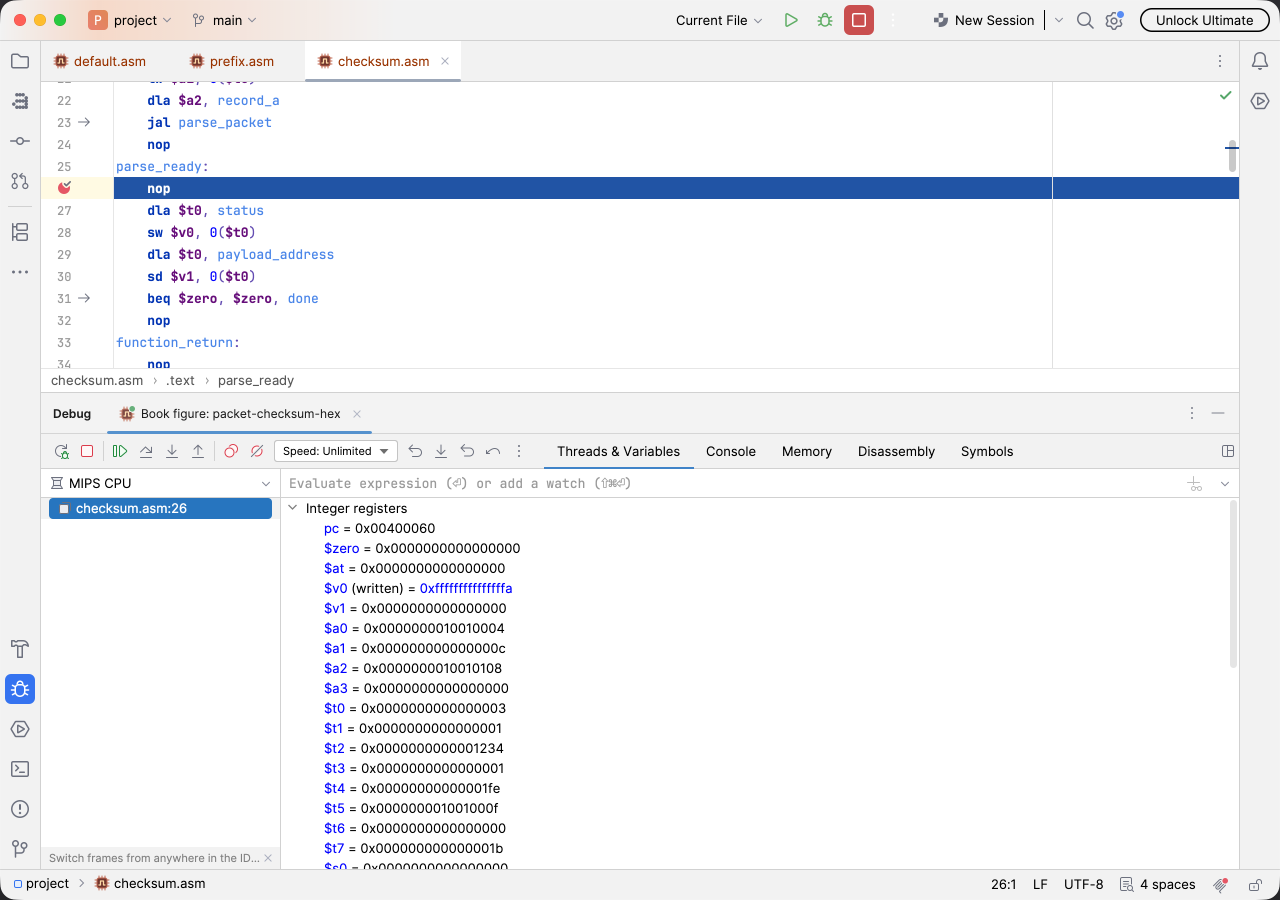
\includegraphics[width=0.42\linewidth,artifact,trim={\MARSpacketchecksumhexLeft{} \MARSpacketchecksumhexBottom{} \MARSpacketchecksumhexRight{} \MARSpacketchecksumhexTop{}},clip]{packages/013-binary-packet-parser/captures/f03-checksum/hex.png}};
    \begin{scope}[shift={(hex.south west)},x={($(hex.south east)-(hex.south west)$)},y={($(hex.north west)-(hex.south west)$)}]
      \draw[black,line width=0.7pt] (0.023437500,0.009708738) rectangle (0.777343750,0.980582524);
      \node[draw=black,fill=white,circle,inner sep=1.5pt,font=\footnotesize] at ($(0.023437500,0.980582524)+(-3mm,0)$) {2};
    \end{scope}
    \node[anchor=north west,inner sep=0,font=\small\bfseries] (decimal-title) at (0.58\linewidth,0 |- hex-title.north) {Signed return values};
    \node[anchor=north west,inner sep=0] (decimal) at ([yshift=-1mm]decimal-title.south west) {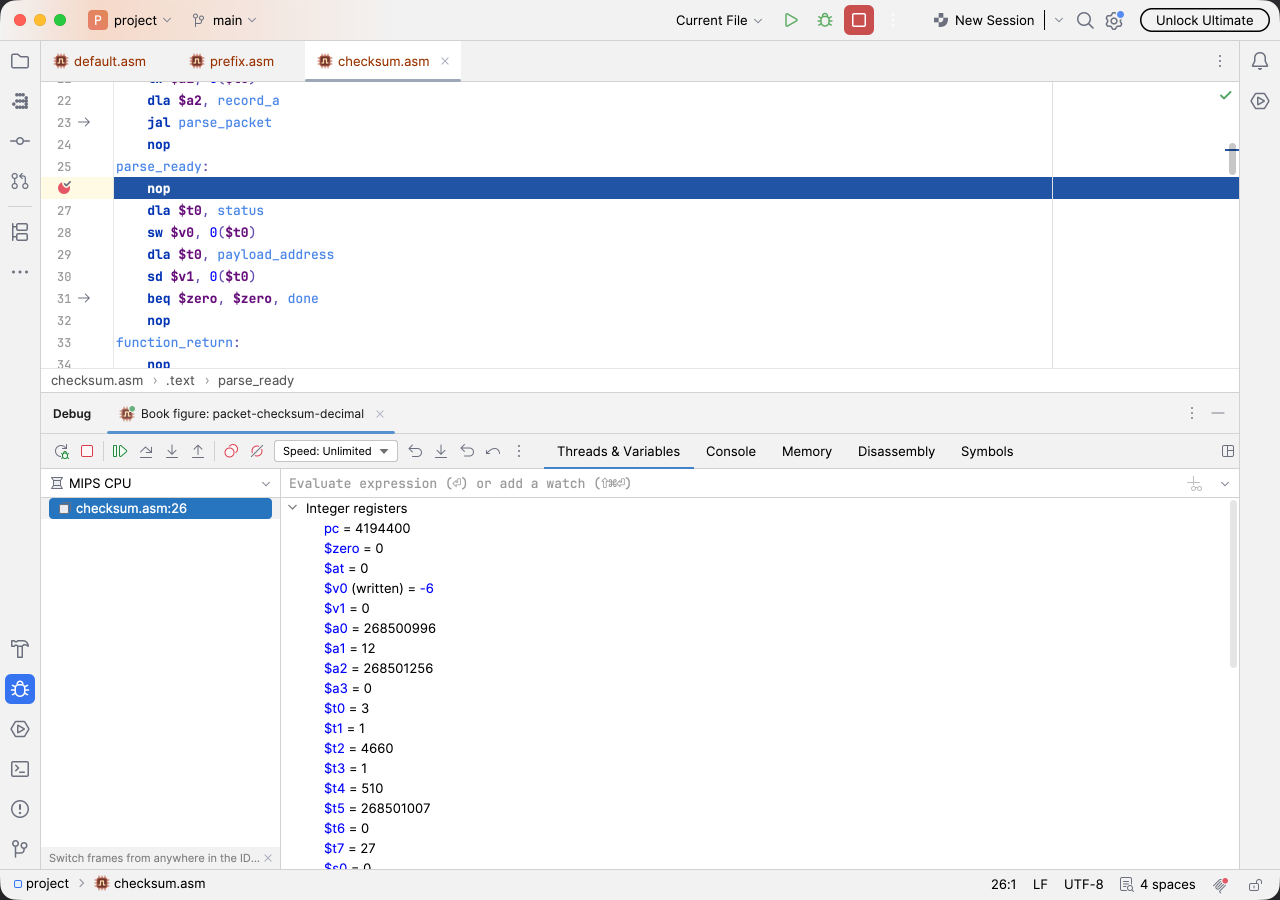
\includegraphics[width=0.42\linewidth,artifact,trim={\MARSpacketchecksumdecimalLeft{} \MARSpacketchecksumdecimalBottom{} \MARSpacketchecksumdecimalRight{} \MARSpacketchecksumdecimalTop{}},clip]{packages/013-binary-packet-parser/captures/f03-checksum/decimal.png}};
    \begin{scope}[shift={(decimal.south west)},x={($(decimal.south east)-(decimal.south west)$)},y={($(decimal.north west)-(decimal.south west)$)}]
      \draw[black,line width=0.7pt] (0.023437500,0.023255814) rectangle (0.468750000,0.953488372);
      \node[draw=black,fill=white,circle,inner sep=1.5pt,font=\footnotesize] at ($(0.023437500,0.953488372)+(-3mm,0)$) {3};
    \end{scope}
    \node[anchor=north west,inner sep=0,font=\small\bfseries] (input-title) at ([yshift=-3mm]hex.south west) {Mapped input bytes, including the preceding guard};
    \node[anchor=north west,inner sep=0] (input) at ([yshift=-1mm]input-title.south west) {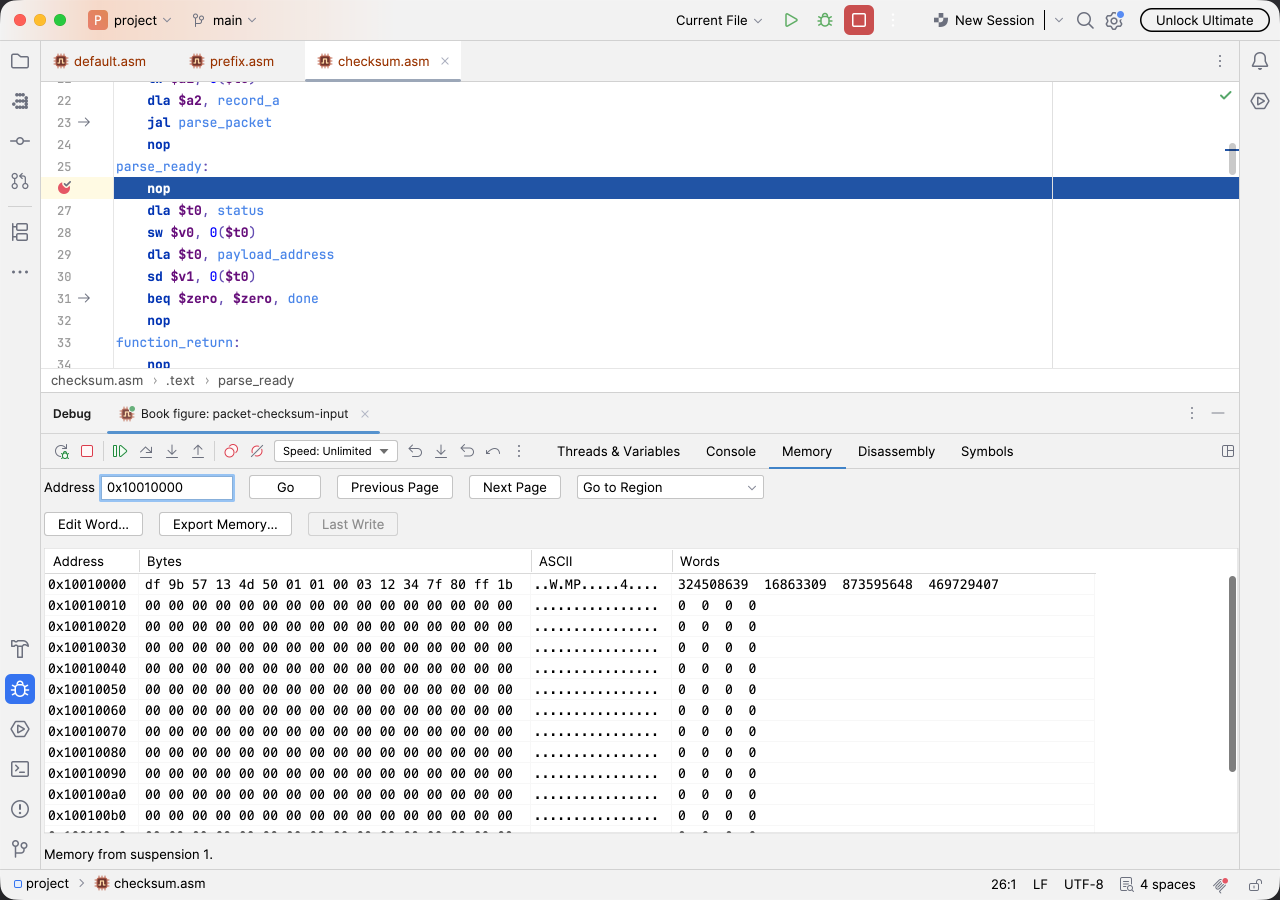
\includegraphics[width=0.84\linewidth,artifact,trim={\MARSpacketchecksuminputLeft{} \MARSpacketchecksuminputBottom{} \MARSpacketchecksuminputRight{} \MARSpacketchecksuminputTop{}},clip]{packages/013-binary-packet-parser/captures/f03-checksum/input.png}};
    \begin{scope}[shift={(input.south west)},x={($(input.south east)-(input.south west)$)},y={($(input.north west)-(input.south west)$)}]
      \draw[black,line width=0.7pt] (0.194672131,0.078431373) rectangle (0.997950820,0.490196078);
      \node[draw=black,fill=white,circle,inner sep=1.5pt,font=\footnotesize] at ($(0,0.490196078)+(-3mm,0)$) {4};
    \end{scope}
    \node[anchor=north west,inner sep=0,font=\small\bfseries] (record-title) at ([yshift=-3mm]input.south west) {Output record and its neighboring words};
    \node[anchor=north west,inner sep=0] (record) at ([yshift=-1mm]record-title.south west) {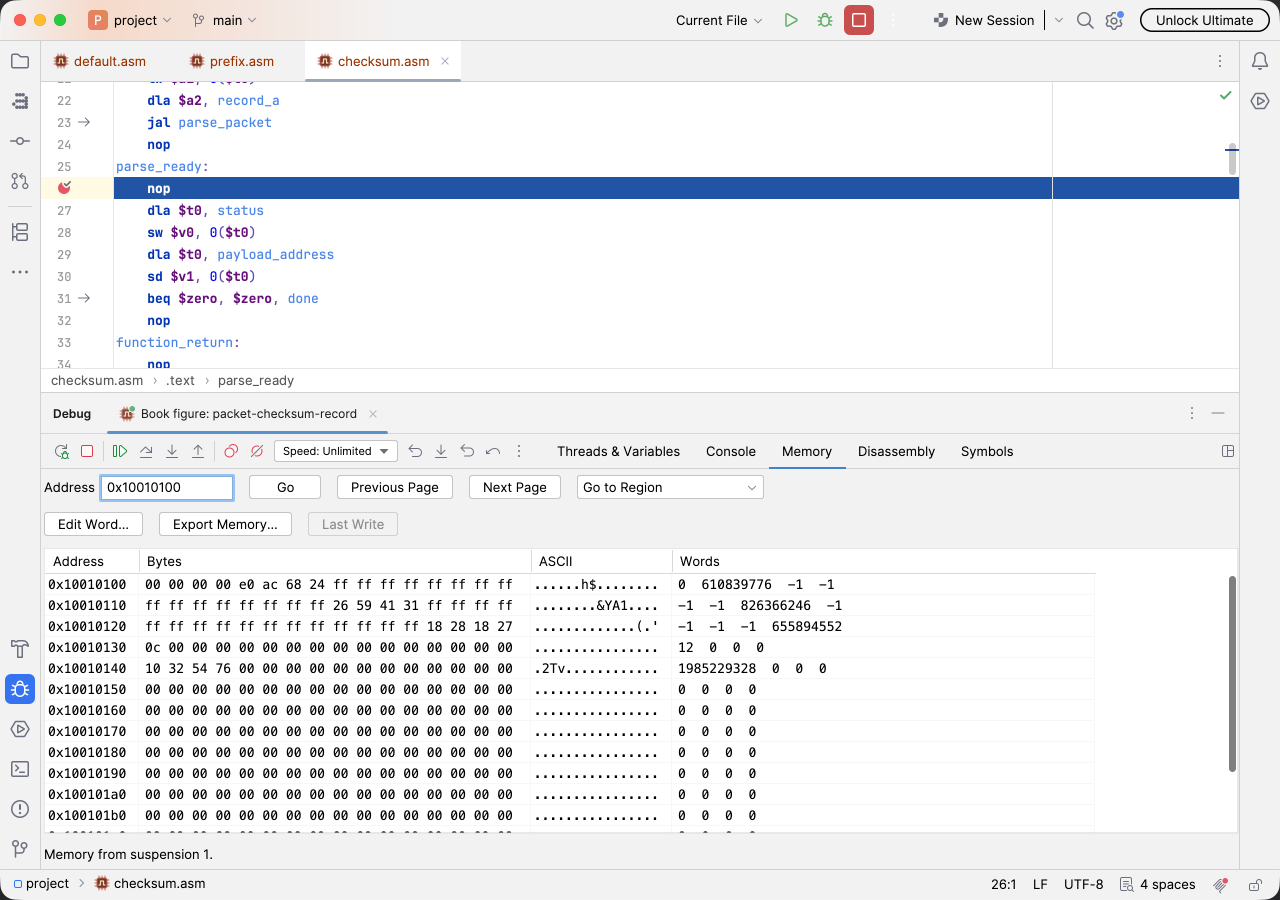
\includegraphics[width=0.84\linewidth,artifact,trim={\MARSpacketchecksumrecordLeft{} \MARSpacketchecksumrecordBottom{} \MARSpacketchecksumrecordRight{} \MARSpacketchecksumrecordTop{}},clip]{packages/013-binary-packet-parser/captures/f03-checksum/record.png}};
    \begin{scope}[shift={(record.south west)},x={($(record.south east)-(record.south west)$)},y={($(record.north west)-(record.south west)$)}]
      \draw[black,line width=0.7pt] (0.194672131,0.055555556) rectangle (0.997950820,0.638888889);
      \node[draw=black,fill=white,circle,inner sep=1.5pt,font=\footnotesize] at ($(0,0.638888889)+(-3mm,0)$) {5};
    \end{scope}
  \end{tikzpicture}
  \par\smallskip
  \begin{minipage}{\linewidth}
    \small
    \begin{enumerate}
      \setlength{\itemsep}{2pt}
            \setlength{\parsep}{0pt}
      \item This fixture changes only the trailer from decimal 26 to 27. The parser has returned to the same \texttt{parse\_ready} boundary, before the caller stores its status and pointer.
      \item \texttt{\$a1 = 0x0c} supplies all twelve required bytes, so this result is not an incomplete prefix. \texttt{\$v0 = 0xfffffffffffffffa} is the sign-extended error value; \texttt{\$v1 = 0} supplies no payload address. Input and output pointers retain their original full-width values.
      \item The native decimal view reports \texttt{\$v0 = -6}, the checksum error. Tentatively decoded fields remain private to the parser until all validation succeeds; the caller receives neither a valid record nor a payload slice on this return.
      \item The final mapped byte is now \texttt{1b}. Header and payload bytes are unchanged, so their unsigned sum is still $232+510=742$. Adding 27 gives 769, whose residue modulo 256 is 1. The required residue is zero. The checksum byte is within the available range in this run.
      \item All four words at \texttt{0x10010108} through \texttt{0x10010117} remain $-1$. Guards and record B are also unchanged. The complete store trace is empty at parser return, proving that no tentative field was written and then restored. Only the caller\textquotesingle s later status and full-width pointer stores follow this marker.
    \end{enumerate}
  \end{minipage}
  \caption{A checksum failure returns minus six and makes no output-record stores.}
  \label{capture:013-binary-packet-parser-f03-checksum}
  \label{packet-f03-checksum}
\end{figure}
\par
